\documentclass[a4paper, 12pt]{article}
\usepackage[T1]{fontenc}
\usepackage[utf8]{inputenc}
\usepackage[left=1in, right=1in, top=1in, bottom=1in]{geometry}
\usepackage[affil-it]{authblk}

\usepackage[format=plain, labelfont={bf,it,large}, textfont={it,large}]{caption}

\usepackage[noend]{algpseudocode}
\usepackage[plain]{algorithm}
\usepackage{algorithmicx}

\usepackage[scaled=0.85]{beramono}
\usepackage[scaled=0.90]{helvet}
\usepackage[tracking=true]{microtype}
\usepackage{amsmath}
\usepackage{amssymb}
\usepackage{amsthm}
\usepackage{bbm}
\usepackage{bm}
\usepackage{bold-extra}
\usepackage{booktabs}
\usepackage{comment}
\usepackage{enumerate}
\usepackage{fancybox}
\usepackage{fontawesome5}
\usepackage{graphicx}
\usepackage{hyperref}
\usepackage{listings}
\usepackage{longtable}
\usepackage{lstbayes}
\usepackage{mathpazo}
\usepackage{mathtools}
\usepackage{multirow}
\usepackage{nicefrac}
\usepackage{scalerel}
\usepackage{setspace}
\usepackage{soul}
\usepackage{sourcesanspro}
\usepackage{subcaption}
\usepackage{tabularx}
\usepackage{textpos}
\usepackage{tgpagella}
\usepackage{tikz}
\usepackage{titlesec}
\usepackage{threeparttable}
\usepackage{varwidth}
\usepackage{xcolor}
\usepackage{xfrac}
\usepackage{xpatch}
\usepackage[shortlabels]{enumitem}

\graphicspath{ {./images/} }

%\counterwithin{figure}{section}
\usetikzlibrary{arrows}
\usetikzlibrary{positioning}

%%%%%%%%%%%%%%%%%%%%%%%%%%%%%%%%%%%%%%%%%%%%%%%%
%%%%%%%%%%%%%%%%%%%bibliography%%%%%%%%%%%%%%%%%%
%%%%%%%%%%%%%%%%%%%%%%%%%%%%%%%%%%%%%%%%%%%%%%%%
\usepackage[backend=biber, style=apa, autocite=inline, doi=false, url=false]{biblatex}
\DeclareLanguageMapping{english}{english-apa}
\setcounter{biburlnumpenalty}{85}  % for urls that are too long
\addbibresource{bibliography.bib}
\renewcommand*{\bibfont}{\footnotesize}
\AtEveryBibitem{%
  % \clearfield{volume}%
  % \clearfield{number}%
  % \clearfield{pages}%
}

\normalem

\onehalfspacing

%%%%%%%%%%%%%%%%%%%%%%%%%%%%%%%%%%%%%%%%%%%%%%%%
%%%%%%%%%%%%%%%%%%%Theorems%%%%%%%%%%%%%%%%%%
%%%%%%%%%%%%%%%%%%%%%%%%%%%%%%%%%%%%%%%%%%%%%%%%
\usepackage[skins,theorems]{tcolorbox}
\tcbset{highlight math style={enhanced,colframe=red,colback=white,arc=0pt,boxrule=1pt}}
\theoremstyle{plain}
\newtheorem{definition}{Definition}
\newtheorem{assumption}{Assumption}
\newtheorem*{unnumdef}{Definition}

\theoremstyle{plain}
\newtheorem{proposition}{Proposition}
\newtheorem{theorem}{Theorem}
\newtheorem{lemma}{Lemma}
\newtheorem{corollary}{Corollary}

\theoremstyle{remark}
\newtheorem*{remark}{Remark}
\newtheorem*{note}{Note}

\makeatletter
\xpatchcmd{\algorithmic}{\itemsep\z@}{\itemsep=1ex plus1pt}{}{}
\makeatother

\newenvironment{proof}[1][Proof]{\noindent\textbf{#1.} }{\ \rule{0.5em}{0.5em}}

\newtheorem{hyp}{Hypothesis}
\newtheorem{subhyp}{Hypothesis}[hyp]
\renewcommand{\thesubhyp}{\thehyp\alph{subhyp}}

\newcommand{\red}[1]{{\color{red} #1}}
\newcommand{\blue}[1]{{\color{blue} #1}}

\newcolumntype{L}[1]{>{\raggedright\let\newline\\arraybackslash\hspace{0pt}}m{#1}}
\newcolumntype{C}[1]{>{\centering\let\newline\\arraybackslash\hspace{0pt}}m{#1}}
\newcolumntype{R}[1]{>{\raggedleft\let\newline\\arraybackslash\hspace{0pt}}m{#1}}

\geometry{left=1.0in,right=1.0in,top=1.0in,bottom=1.0in}

\begin{document}

\begin{titlepage}
\title{\textbf{Final Term Paper} \\[1ex] \large Topics in Econometrics and Statistics, Summer Term 2022 }
\author{Chencheng Fang\thanks{Email: \href{mailto: ccfang@uni-bonn.de}{ccfang[at]uni-bonn.de}, Bonn Graduate School of Economics} \\ \small (Matriculation Number: 3466204)}
\date{\today}
\maketitle
\begin{abstract}
\onehalfspacing
\noindent In this essay, I introduce the main insights in \cite{Bauer2019} and contributions it makes to the existing literature. I try to replicate the simulation in that paper, and thus verify the advantage of its newly proposed approach over alternatives at certain circumstances. I also find some other interesting facts that the paper somewhat ignores, and design a simple interactive web app to visualize the out-of-sample prediction accuracy of those approaches. All materials I create for this project can be found on my \href{https://github.com/ccfang2/TopicsMetricsStats2022}{GitHub}. There is no guarantee that I fully understand the new approach and precisely reproduce the simulation. Interested readers are strongly recommended to read the original paper.\\


\bigskip
\end{abstract}
\setcounter{page}{0}
\thispagestyle{empty}
\end{titlepage}
\pagebreak \newpage




\doublespacing


\section{Introduction}
\label{sec:introduction}

This essay establishes on the paper entitled \textit{"On deep learning as a remedy for the curse dimensionality in nonparametric regression"} by \cite{Bauer2019}. In that paper, it is proved that least squares estimates constructed from multilayer feedforward neural networks are able to circumvent the curse of dimensionality in nonparametric regression as long as a smoothness condition and a suitable restriction on the structure of regression function hold. 

Contrary to parametric approach, the regression function in nonparametric approach is not claimed to be characterized by finitely many parameters, so the whole function is data driven. Moreover, as claimed by \cite{Gyoerfi2002}, one has to restrict the class of regression functions when considering the rate of convergence. Thus, \cite{Bauer2019} introduce the definition of $(p,C)$-smoothness. One can simply take $p$ as the degree of smoothness even though they are slightly different. \cite{Stone1982} shows that the optimal minimax rate of convergence for estimating a $(p,C)$-smooth regression function is $n^{-\frac{2p}{2p+d}}$, where $d$ is the dimensionality of input. Apparently, the rate of convergence can be exceedingly small when $d$ is comparatively large to $p$, and this property is the so-called curse of dimensionality.

Much endeavor has been made to bypass this problem. \cite{Stone1985} adds an additivity condition to the structure of regression function, and the resulting model is a sum of $(p,C)$-smooth univariate functions $m_1,\ldots,m_d: \mathbb{R} \rightarrow \mathbb{R}$. \cite{Stone1985} shows that $n^{-\frac{2p}{2p+1}}$ is the optimal minimax rate of convergence in this occasion. \cite{Stone1994} further generalizes it to an interaction model, which allows the existence of interaction terms in smooth functions. He proves that the optimal minimax rate of convergence then becomes $n^{-\frac{2p}{2p+d^{*}}}$ where $d^{*}  \in \{1,\ldots,d\}$ is the number of interaction terms. 

Another stream of research takes account of the so-called single index model, where the $d$ dimensions of input are firstly linearly combined and then transformed by a univariate function (e.g., \cite{Hardle1993}). This idea is extended to the well-known projection pursuit, where the function is a sum of functions of those in single index model (e.g., \cite{Friedman1981}). It is demonstrated that if the univariate functions in above models are $(p,C)$-smooth, the regression estimates can reach the univariate rates of convergence (i.e., $n^{-\frac{2p}{2p+1}}$) up to some logarithmic factor (e.g., \cite{Gyoerfi2002}). Furthermore, \cite{Horowitz2007} also consider a regression model where the innermost layer is a sum of smooth functions, each of which takes a single component of $d$ dimensional inputs as its own input, and the output of inner layer is then recursively used as input of outer layer. They show a univariate rate of $n^{-\frac{2p}{2p+1}}$ in such model with the use of a penalized least squares estimate for smoothing splines.

\cite{Bauer2019} argue that, even though the above models can achieve a satisfactory rate of convergence, it is only possible with the imposed strict assumptions being satisfied. Thus, they aim to derive rates of convergence for more general forms of functions, which approximate the real world better and are hopefully simpler. In their paper, they propose a model of multilayer feed-forward neural networks, which not only cleverly imitate the property of modularity in real-world complex technical systems, but also utilize the advantage of using neural networks in high dimensional occasions. \cite{Bauer2019} contributes to the existing literature body by proving an achievable rate of convergence irrespective of $d$ in their model and meanwhile allowing $p$ in $(p,C)$-smooth regression functions to be larger than 1. This greatly relaxes the assumptions of precedent models.

The rest of essay is organized as follows. Section \ref{sec:review} reviews the statistical model and some important theorems from the paper. In Section \ref{sec:simulation}, Monte-Carlo simulations are carried out and in Section \ref{sec:shiny}, an R Shiny app is designed to interactively visualize the performance of the model and other alternatives. Section \ref{sec:conclusion} concludes this essay.
\section{Review}
\label{sec:review}

The newly proposed model of multilayer feed-forward neural networks in \cite{Bauer2019} is built on a generalized hierarchical interaction model with neural networks as a technique to approximate regression functions. 

\subsection{Generalized Hierarchical Interaction Model}

The generalized hierarchical interaction model is analogous to complex technical system in terms of modularity. \cite{Kohler2017} gives its mathematical definition, as shown in Definition \ref{def1}.

\begin{definition}
Let $d \in \mathbb{N}$, $d^* \in \{1,\ldots,d\}$ and $m:\mathbb{R}^d \rightarrow \mathbb{R}$.
\begin{enumerate}[(a)]
    \item We say that $m$ satisfies a generalized hierarchical interaction model of order $d^*$ and level 0, if there exist $a_1,\ldots,a_{d^*} \in \mathbb{R}^d$ and $f:\mathbb{R}^{d^*}\rightarrow \mathbb{R}$ such that for all $x \in \mathbb{R}^d$, 
    \[ m(X)=f(a_1^TX,\cdots,a_{d^*}^TX) \]
    \item We say that $m$ satisfies a generalized hierarchical interaction model of order $d^*$ and level $l+1$, if there exists $K\in \mathbb{N}$, $g_k:\mathbb{R}^{d^*} \rightarrow \mathbb{R}(k=1,\cdots,K)$ and $f_{1,k},\cdots,f_{d^*,k}: \mathbb{R}^d \rightarrow \mathbb{R} (k=1,\cdots,K)$ such that $f_{1,k},\cdots,f_{d^*,k} (k=1,\cdots,K)$ satisfy a generalized hierarchical interaction model of order $d^*$ and level $l$, and for all $X \in \mathbb{R}^d$,
    \[ m(X)=\sum_{k=1}^{K}g_k(f_{1,k}(X),\cdots,f_{d^*,k}(X))\]
    \item We say that the generalized hierarchical interaction model defined above is $(p,C)$-smooth, if all functions occurring in its definition are $(p,C)$-smooth according to Definition \ref{def1}.
\end{enumerate}
\label{def1}
\end{definition}

In compliance with Definition \ref{def1}, the aforementioned single index model belongs to generalized hierarchical interaction models with order 1 and level 0, while additive model and projection pursuit have order 1 and level 1. Now, it comes to the question of how to estimate those functions in the model?

\subsection{Multilayer Feedforward Neural Network}

The application of neural networks in high dimensional case becomes increasingly popular in recent years. \cite{Bauer2019} propose to use neural networks to estimate regression functions in the above-mentioned generalized hierarchical interaction models. But, what about the rate of convergence in such models?

Existing literature on neural network regression estimates has extensively studied their rates of convergence. In respect of single hidden layer neural network, \cite{Barron1994} shows that its $L_2$ error has a dimensionless rate of $n^{-1/2}$ (up to some logarithmic factor), provided the Fourier transform has a finite first moment. \cite{McCaffrey1994} prove that the $L_2$ error has a rate of $n^{-\frac{2p}{2p+d+5}+\epsilon}$ when the single hidden layer neural network estimate for $(p,C)$-smooth functions is suitably defined. In terms of two- or multi-layer neural networks, \cite{Kohler2005} find that suitable two layer neural network estimates can achieve a rate of $n^{-\frac{2p}{2p+d^*}}$ (up to some logarithmic factor) for $(p,C)$-smooth interaction models with $p \le 1$, so the convergence rate is associated with $d^*$, the order of model, instead of $d$, the dimension of input. In \cite{Kohler2017}, the finding is further extended to suitably defined multi-layer neural networks, but the condition of $p \le 1$ is still imposed.

A main contribution in \cite{Bauer2019} is that they design sets of multilayer feedforward neural networks according to generalized hierarchical interaction models, and define regression estimates as least squares estimates based on this class of neural networks. In their neural networks, they relax the condition of $p$ and allow it to be larger than 1 while maintaining a $d$-irrelevant rate of $n^{-\frac{2p}{2p+d^*}}$ (up to some logarithmic factor). With this less stringent condition, one can utilize $p$, the degree of smoothness, to speed up convergence. The precise definition of multilayer feedforward neural networks is given in Definition \ref{def2} as follows.

\begin{definition}
Let $K$, $d^*$, $d$ and $l$ has the same meaning as those in Definition \ref{def1}, and let $M^*$ be a parameter introduced for technical reasons and originating from the composition of several smaller networks in proof of that paper. It controls the accuracy of approximation. 

\begin{enumerate}[(a)]
    \item For $M^* \in \mathbb{N}$, $d \in \mathbb{N}$, $d^* \in \{1,\ldots, d\}$ and $\alpha >0$, we denote the set of all functions $f: \mathbb{R}^d \rightarrow \mathbb{R}$ that satisfy:
    \[f(X) = \sum_{i=1}^{M^*}\mu_i \cdot \sigma \left( \sum_{j=1}^{4d^*} \lambda_{i,j}\cdot \sigma\left(\sum_{v=1}^{d} \theta_{i,j,v}\cdot X^{(v)} +\theta_{i,j,0}\right) +\lambda_{i,0} \right)+\mu_0\]
    $(X \in \mathbb{R}^d)$ for some $\mu_{i}$, $\lambda_{i,j}$ and $\theta_{i,j,v} \in \mathbb{R}$, where $|\mu_i|\le\alpha$, $|\lambda_{i,j}|\le\alpha$ and $|\theta_{i,j,v}|\le\alpha$ for all $i \in \{0,1,\ldots, M^*\}$, $i \in \{0,\ldots,4d^*\}$, $v \in \{0,\ldots,d\}$, by $\mathcal{F}_{M^*,d^*,d,\alpha}^{(\textsf{neural networks})}$.
    \item For $l=0$,we define our space of hierarchical neural networks by \[\mathcal{H}^{(0)}=\mathcal{F}_{M^*,d^*,d,\alpha}^{(\textsf{neural networks})}\]
    For $l>0$, we define recursively \[ \mathcal{H}^{(l)}=\left\{h:\mathbb{R}^d \rightarrow \mathbb{R}: h(X)=\sum_{k=1}^K g_k(f_{1,k}(X),\ldots,f_{d^*,k}(X))\right\}\] 
    for some $g_k \in \mathcal{F}_{M^*,d^*,d^*,\alpha}^{(\textsf{neural networks})}$ and $f_{j,k} \in \mathcal{H}^{(l-1)}$
    \item We define $\tilde{m}_n$ as the least squares estimate \[\tilde{m}_n(\cdot)=\arg\min_{h\in\mathcal{H}^{(l)}}\frac{1}{n}\sum_{i=1}^n|Y_i-h(X_i)|^2\]
\end{enumerate}
\label{def2}
\end{definition}

As per Definition \ref{def2}, components of a function from $\mathcal{H}^{(l)}$ is illustrated in Figure \ref{fig1}. Moreover, an example of multilayer feedforward neural network with $l=1$,$K=2$,$d=7$,$d^*=2$ and $M^*=2$ is displayed in Figure \ref{fig2}. It can be seen that this class of neural networks is sparsely connected, as contrast to fully connected neural networks in existent literature. This better reflects the modularity of systems which is prevalent in real world. Also, with less weights, the estimation of sparse networks can be more efficient. Although the number of weights can still be very large with increasing number of layers, it can be contained because a typical example of technical systems usually have a moderate finite $l$. The major result of such neural networks that \cite{Bauer2019} find is in Theorem \ref{theorem1}.

\begin{theorem}
Let $(X,Y), (X_1, Y_1),\ldots, (X_n,Y_n)$ be iid random variables with values in $\mathbb{R}^d \times \mathbb{R}$ such that supp$(X)$ is bounded and \[\mathbf{E} \quad exp(c_1 \cdot Y^2)<\infty\] for some constant $c_1>0$.Let $m$ be the corresponding regression function satisfying a $(p,C)$-smooth generalized hierarchical interaction model of order $d^*$ and finite level $l$ with $p=q+s$ for some $q\in \mathbb{N}_0$ and $s \in (0,1]$. Let $N\in\mathbb{N}_0$ with $N\ge q$. Furthermore, assume that in Definition \ref{def1}(b) all partial derivatives of order less than or equal to $q$ of the functions $g_k$,$f_{j,k}$ are bounded, that is, assume that each such function $f$ satisfies \[\max_{j_1,\ldots,j_d\in\{0,1,\ldots,q\},\\ j_1+\ldots,+j_d\le q} \| \frac{\partial^{j_1+\ldots,+j_d}f}{\partial^{j_1}x^{(1)}\cdots \partial^{j_d}x^{(d)}}\| \le c_2\]
and let all functions $g_k$ be Lipschitz continuous with Lipschitz constant $L>0$ [which follows from if $q>0$]. Let $\mathcal{H}^{(l)}$ be defined with $K,d,d^*$ as in Definition \ref{def2}, $M^*=\lceil c_{56}\cdot n^{\frac{d^*}{2p+d^*}}\rceil, \alpha=n^{c_{57}}$ for sufficiently large constants $c_{56},c_{57}>0$ and using an N-admissible $\sigma:\mathbb{R} \rightarrow [0,1]$. Let $\tilde{m_n}$ be least squares estimate and $m_n=T_{c_3 \cdot log(n)}\tilde{m_n}$. Then, \[\mathbf{E}\int|m_n(x)-m(x)|^2\mathbf{P}_X(dx)\le c_4 \cdot log(n)^3 \cdot n^{-\frac{2p}{2p+d^*}}\] holds for sufficiently large n.
\label{theorem1}
\end{theorem}

As shown in Theorem \ref{theorem1}, for multilayer feedforward neural networks, the $L_2$ error has a rate of convergence at $n^{-\frac{2p}{2p+d^*}}$ up to some logarithmic factor. The rate is not related to $d$, the dimension of input, but $d^*$ of input components. Also, $p\ge 1$, which greatly relaxes the strict condition in previous neural network models. With this relaxed condition, one can fully utilize $p$, the degree of smoothness, to expedite convergence. One noteworthy drawback is that some parameters (e.g., $l$, $K$ or $d^*$) of the estimate $m_n$ is unknown, so the choice of them is data-dependent and can be very time consuming.
\section{Simulation}
\label{sec:simulation}

In this section, I use Monte-Carlo simulation to test if the newly proposed model in \cite{Bauer2019} performs better than alternative models in varying cases. My setup here is almost the same as that of original paper, but simpler. I will not reiterate all details of my setup but only mention the differences from that of original paper.

\begin{enumerate}[(a)]
    \item I don't use all functions that they use for data generation. Since $m_1$, $m_2$ and $m_3$ all represent ordinary general hierarchical interaction models, I use $m_1$ and $m_2$ as an examples. I also include $m_4$ and $m_5$ to analyze the conditions of $d^*=1$ and $d^*=d$, respectively.
    \item In terms of prediction models, I only concern with simple nearest neighbor estimate (\textit{neighbor/knn}), interpolation with radical basis function (\textit{RBF}), fully connected neural network with one hidden layer (\textit{neural-1}) and multilayer feedforward neural networks defined in Definition \ref{def2} (\textit{neural-x}). I abandon \textit{neural-3} and \textit{neural-6} for consideration of time efficiency because I use R programming which is not very machine learning friendly. But I add a random forest model (\textit{rf/random forest}) as an alternative.
    \item For the parameter $k_n$ in simple nearest neighbor estimate, I don't adaptively select it from a set of values, and instead choose the value of 4 discretionarily. Otherwise, it would take too much time to run the whole batch of codes in R.
    \item Again for consideration of time efficiency, I reduce the sample size of test data from $100000$ to $500$, and also scale down the repeating times of simulation from $50$ to $10$.
    \item I also simulate a simpler version of multilayer feedforward neural networks, which is clarified and explained later.
\end{enumerate}

Before proceeding to simulating the multilayer feedforward neural networks, I summarize Algorithm \ref{alg1} as follows, with reference to Definition \ref{def2} and simulation setup in \cite{Bauer2019}.

\begin{tcolorbox}[standard jigsaw, opacityback=0]
\begin{algorithm}[H]
\caption{Multilayer feedforward neural networks}
\label{alg1}
\begin{algorithmic}[1]
\State define $d$ as the dimension of input
\For {each $d^*$ in $\{1,\ldots,d\}$}
\For {each $M^*$ in $\{1,\ldots,5,6,11,16,21,\ldots,46\}$}
\State construct neural networks with $d^*$, $M^*$ and $l=0$:$\mathcal{H}^{(0)}$
\State estimate $L_2$ error of neural network with $d^*$, $M^*$ and $l=0$
\For {each $l$ in $\{1,2\}$}
\For {each $K$ in $\{1,\ldots,5\}$}
\State construct neural networks with $d^*$, $M^*$, $l=1$ or $2$ and $K$: $\mathcal{H}^{(l)}$
\State estimate $L_2$ error of neural network with $d^*$, $M^*$, $l$ and $K$
\EndFor
\EndFor
\EndFor
\EndFor
\State find the minimum $L_2$ error and the corresponding neural network
\end{algorithmic}
\end{algorithm}
\end{tcolorbox}

I make much attempt to code this algorithm in R, but there are so many large neural networks to run and R programming is not very efficient in estimating neural networks. So, I decide to just estimate neural network with $l=0$, in a hope that if neural network with $l=0$ performs well, the multilayer feedforward neural networks selected by Algorithm \ref{alg1} can only function better. Table \ref{table1} presents my Monte-Carlo simulation \footnote{If one gets a warning \textit{Algorithm did not converge in 1 of 1 repetition(s) within the stepmax} when running my code, please increase the value of parameter \textit{stepmax} or adjust parameter \textit{threshold} in function \textit{neuralnet}} result, and it corroborates the findings in \cite{Bauer2019}.

\begin{enumerate}[(a)]
\item In cases of $m_1$ and $m_2$, i.e., ordinary hierarchical interaction model, and when disturbance of noise is weak, i.e., $\sigma=5\%$, the new approach has the smallest scaled empirical $L_2$ error among all models concerned. Moreover, I only use neural network with $l=0$ in simulation for consideration of time, so neural network sorted out by Algorithm \ref{alg1} can perform even better. When disturbance of noise is strong, i.e., $\sigma=20\%$, the performance of new approach ranks the second, and can still be considered as decent. There is a high chance that the new approach can be the best if I successfully implement Algorithm \ref{alg1}.

\item In case of $m_4$, i.e., additive model with $d^*=1$ and $m_5$, i.e., interaction model with $d^*=d$, and when noise is weak, the new approach performs the second best and the best, separately. Moreover, when noise is strong, even though it fails to be the best, it still functions well enough, giving out a relatively small scaled empirical $L_2$ error. Our finding is consistent with \cite{Bauer2019}.
\end{enumerate}

Besides, I have also witness two other interesting new facts from my simulation. 

\begin{enumerate}[(a)]
\item I record the time duration consumed in simulation for each case, and I find out it takes much more time to run simulation for $m_1$ and $m_2$ (more than 1 hour), while it is way faster to run codes for $m_4$ and $m_5$ (less than 1 minute). In case of $m_4$, because $d^*=1$, then rate of convergence $n^{-\frac{2p}{2p+d^*}}$ can be very high, and the algorithm converges speedily. In case of $m_5$, an exponential function, despite the fact that $d^*=d$, the degree of smoothness, $p$, can be fully taken advantage of to speed up convergence. 
\item I also discover that when the disturbance of noise in data generation process increase from $5\%$ to $20\%$, the scaled empirical $L_2$ error grows. This might be due to the fact that with more noise, the property of modularity imbedded in data structure is impaired more, and the prediction power of the new approach is thus weakened.
\end{enumerate}
\section{Shiny App in R}
\label{sec:shiny}

In this section, I design an R shiny app to interactively visualize the prediction power of multilayer feedforward neural network and other alternative models. The server logic of this app is almost the same as that in Section \ref{sec:simulation}. However, to expedite the reaction of my app, I only run a single simulation each time a set of parameters are given, instead of running multiple simulations and calculating the average. Sample size of test dataset is also decreased to 200. My web app is designed in \href{https://shiny.rstudio.com}{Shiny RStudio} and can be simply accessed by clicking this \href{https://ccfang2.shinyapps.io/neuralxSim/}{link}\footnote{This app is invalidated every 25 hours. Hence, if you could not open this link, please go to my \href{https://github.com/ccfang2/TopicsMetricsStats2022}{GitHub} for further instructions.}.

Figure \ref{fig3} displays the layout of my Shiny app. This app needs to be bundled with this essay since terminologies or models are not explained in detail on the webpage, but all can be traced in this essay. The usage is summarized as follows.

\begin{enumerate}[(a)]
    \item Select a function for generating data. I only consider $m_1$, $m_2$, $m_4$ and $m_5$, the same as in Section \ref{sec:simulation}. The default function is $m_4$.
    \item Select the degree of noise disturbance in data generation, i.e., $\sigma=5\%$ or $20\%$. The default is $5\%$.
    \item Select all models you want to build and compare with each other. I exclude interpolation method of radial basis function because there is something wrong in my code which I fail to debug for now. The default model is simple nearest neighbor estimate.
    \item Click the button "Run", and then three plots will pop out, which helps us to compare between different models. It is noteworthy that one may need to wait a few minutes for the output to come when $m_1$ and $m_2$ are selected.
    \item Click the button "Run" again to observe another simulation result with the same given inputs.
    \item Re-select a function, degree of noise disturbance or models to observe simulation result with different inputs.
    \item Refresh the web page to reset this app.
\end{enumerate}

Figure \ref{fig4} presents an example of output plots with $m_1$, $5\%$ and all four models. There are three subplots, each of which explains the prediction accuracy from a distinct angle. The top subplot depicts the prediction errors of models, from which I can generally recognize that the neural network with one hidden layer and the multilayer feedforward neural network perform better than the other two. The bottom left subplot is a bar plot showing the scaled empirical $L_2$ error of each model, from which I clearly know the new approach predicts the most accurately and simple nearest neighbor model is the worst. Finally, the bottom right subplot is a correlation matrix plot, which visualizes the correlation between true target value in test dataset and predicted value of each model. All correlations are positive, and the size of circle indicates the strength of correlation. Again, it is obvious the correlation reaches the highest when the new approach is concerned.

\section{Conclusion}
\label{sec:conclusion}

In this essay, I first introduce the critical insights and contributions \cite{Bauer2019} make to the existing literature. I then review the precise statistical model of multilayer feedforward neural network and the motivation behind this model. I also notify how this new model differs from previous models and its improvement upon others. To follow up, I attempt to replicate the Monte-Carlo simulation in the original paper. Even though my simulation is simpler, my simulation results are still reconcilable with theirs in a sense that multilayer feedforward neural networks perform extraordinarily in cases of ordinary general hierarchical interaction models with $1<d^*<d$. Furthermore, I point out two new interesting findings on basis of my simulation. Finally, I design an R Shiny App to visualize the prediction power of all models in an interactive way. 


\section*{Acknowledgement}
I thank Joachim Freyberger, the lecturer of this course, for his insightful comments and instructions in helping me understand the original paper. I am also grateful to Tim Mensinger for the LaTeX template he uploaded to his \href{https://github.com/timmens/topics-metrics-2021}{GitHub}, which I use to compile this essay. Last but not least, I thank \cite{Bauer2019} for their amazing work. It is worthy of mentioning that there is no guarantee I fully comprehend their paper, so readers who are interested are strongly encouraged to read their paper. Discussions are always welcomed though.

\singlespacing
\setlength\bibsep{0pt}



\clearpage

\onehalfspacing

\newpage

\begin{table}

    \centering
    
    \caption{Simulation Results}
    \label{table1}
    \resizebox{\textwidth}{!}{%
\begin{tabular}{c||c|c}
    \hline
	& \multicolumn{2}{c}{$m_1$} \\
	\hline
	& 5\% & 20\% \\
	\hline
	& Median(IQR)&Median(IQR)\\
	\hline
	KNN & 0.5821 (0.1395) & 0.5032 (0.0775) \\
	\hline
	RBF^\star & 0.6270 (116.6120) & 0.6597 (943.0001) \\
	\hline
	Random Forest & 0.5283 (0.1041) & 0.5793 (0.1357) \\
	\hline
	Neural-1 & 0.2163 (0.4285) & \textbf{0.3485 (0.4204)} \\
	\hline
	Neural-x & \textbf{0.1765 (0.0919)} & 0.4889 (0.3356) \\
	\hline
	& \multicolumn{2}{c}{$m_2$} \\
	\hline
	KNN & 0.8870 (0.1164) & 0.8385 (0.0226) \\
	\hline
	RBF^\star & 0.7941 (0.0448) & 0.7547 (0.0848) \\
	\hline
	Random Forest & 0.4587 (0.1098) & 0.4307 (0.1530) \\
	\hline
	Neural-1 & 0.3672 (0.1257) & \textbf{0.2277 (0.1752)} \\
	\hline
	Neural-x & \textbf{0.3217 (0.1840)} & 0.3509 (0.2407) \\
	\hline
	& \multicolumn{2}{c}{$m_4$} \\
	\hline
	KNN & 0.2495 (0.0324) & 0.3219 (0.0278) \\
	\hline
	RBF^\star & 0.2592 (0.3233) & 0.2030 (0.1387) \\
	\hline
	Random Forest & 0.2563 (0.0374) &  0.3209 (0.0382) \\
	\hline
	Neural-1 & \textbf{0.0244 (0.0089)} & \textbf{0.1603 (0.0223)} \\
	\hline
	Neural-x & 0.0303 (0.0130) & 0.2470 (0.0308) \\
	\hline
	& \multicolumn{2}{c}{$m_5$} \\
	\hline
	KNN & 0.2579 (0.0440) & 0.3228 (0.0404) \\
	\hline
	RBF^\star & 0.1815 (0.2798) & 0.3341 (0.3949) \\
	\hline
	Random Forest & 0.3605 (0.0406) & 0.4064 (0.0400) \\
	\hline
	Neural-1 & 0.0717 (0.0353) & \textbf{0.1756 (0.0303)} \\
	\hline
	Neural-x & \textbf{0.0492 (0.0186)} & 0.2122 (0.0576) \\
	\hline
\end{tabular}
 }
 \begin{tablenotes}
      \normalsize
      \item  ${}^\star$ Please be aware that there are some bugs in my simulation of RBF model, and I fail to debug them before the deadline of the project.
    \end{tablenotes}

\end{table}

\clearpage
\newpage

\begin{figure}[hp]
  \centering
  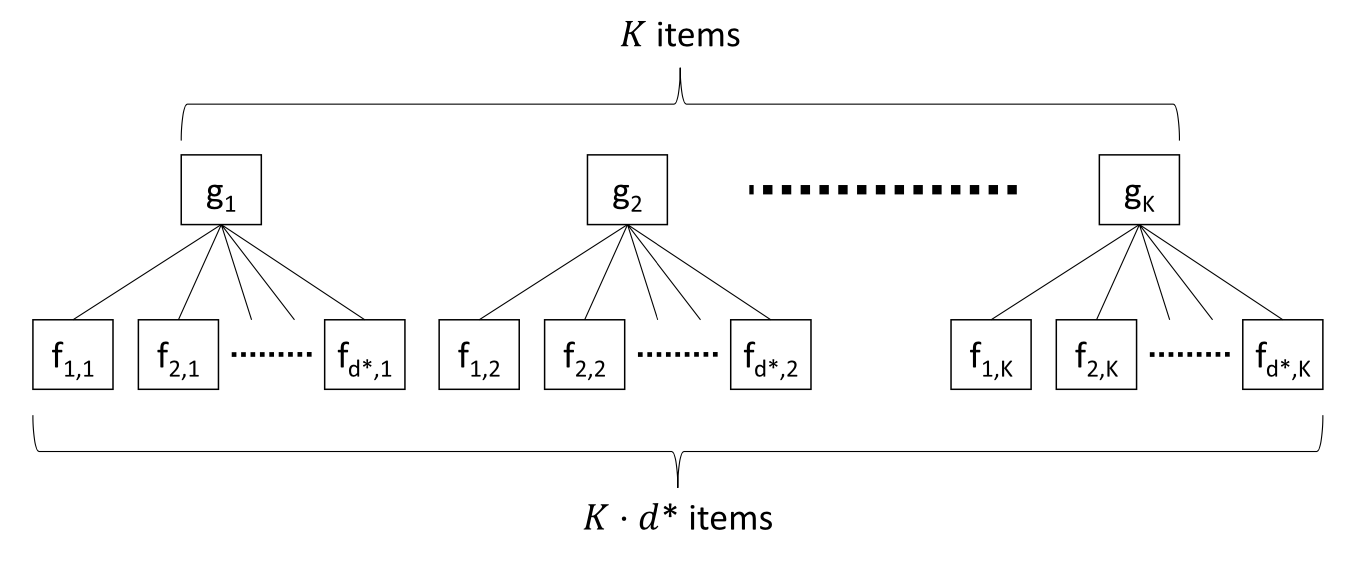
\includegraphics[scale=0.7]{figure1.png}
  \caption{Illustration of components of a function from H(l)}
  \floatfoot{\normalsize{Note: From \cite{Bauer2019}}}
  \label{fig1}
\end{figure}

\clearpage
\newpage

\begin{figure}[hp]
  \centering
  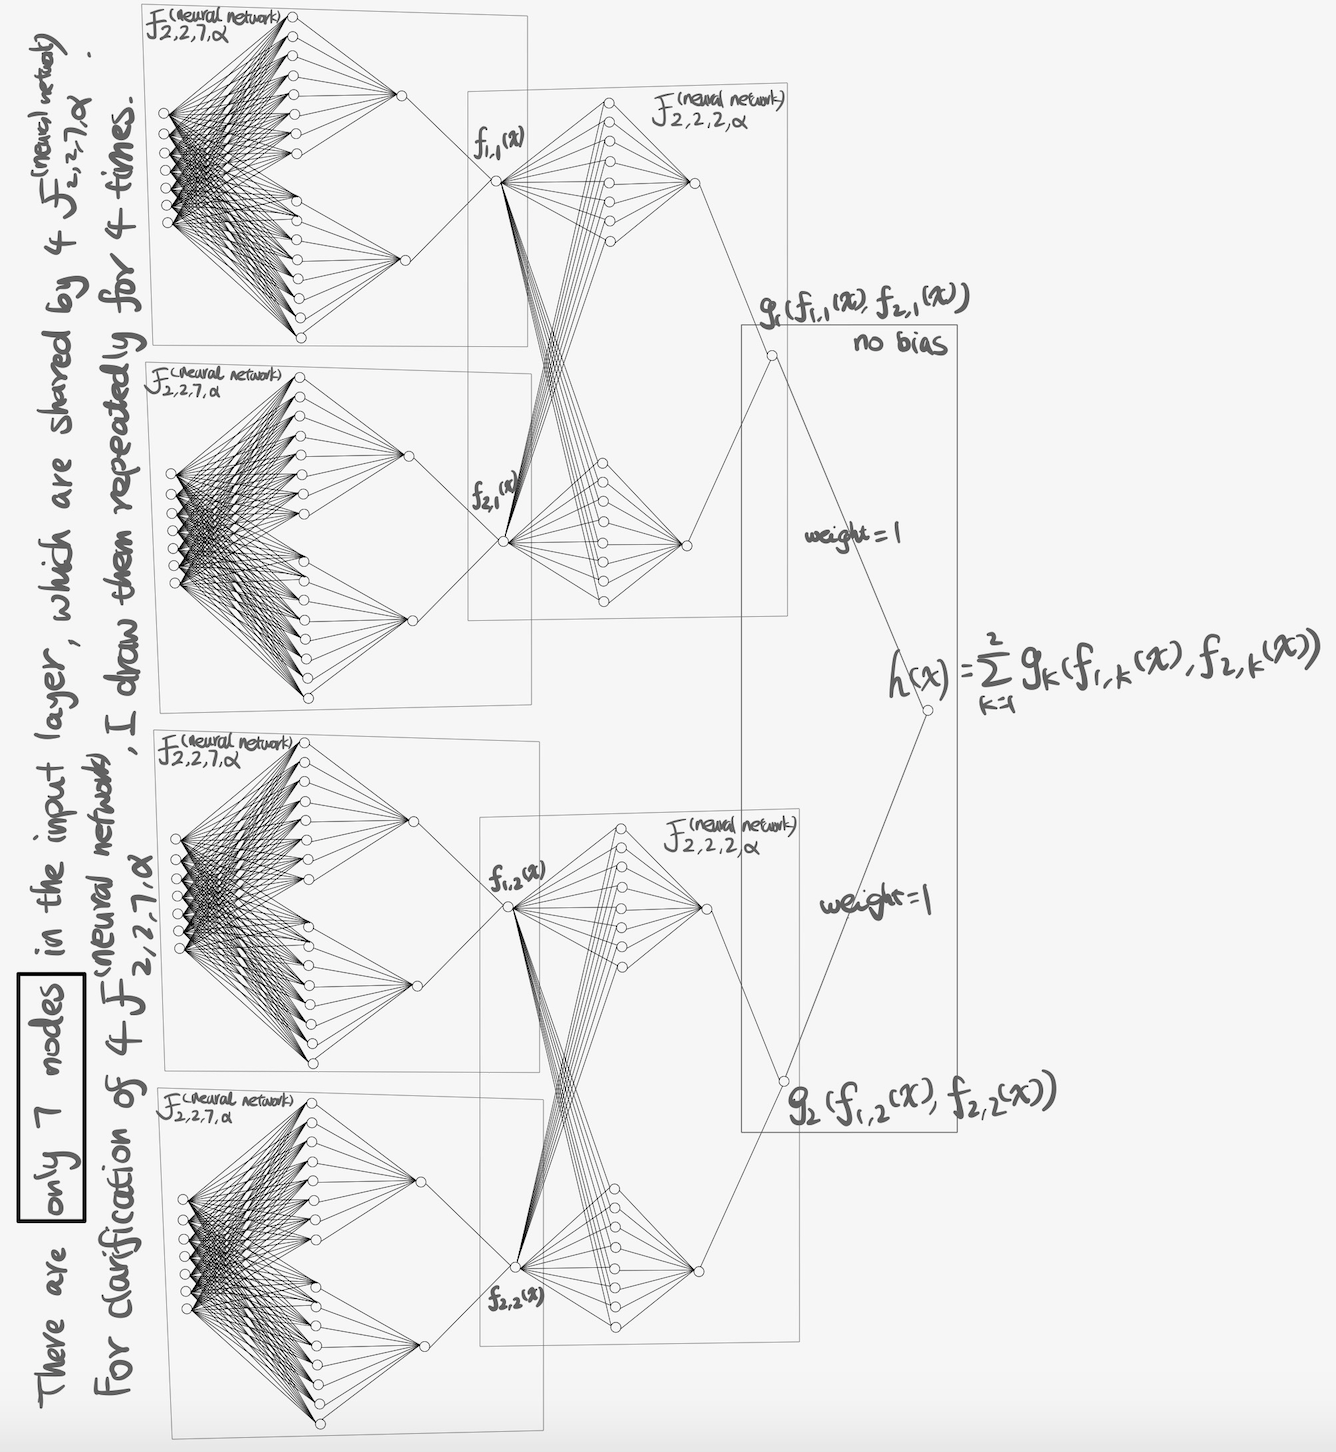
\includegraphics[scale=0.75]{figure2.png}
  \caption{Example of multilayer feedforward neural network}
  \floatfoot{\normalsize{Note: There are only 7 nodes in the input layer, which are shared by the 4 neural networks. For convenience, I draw them separately for 4 times}}
  \label{fig2}
\end{figure}

\clearpage
\newpage

\begin{figure}[hp]
  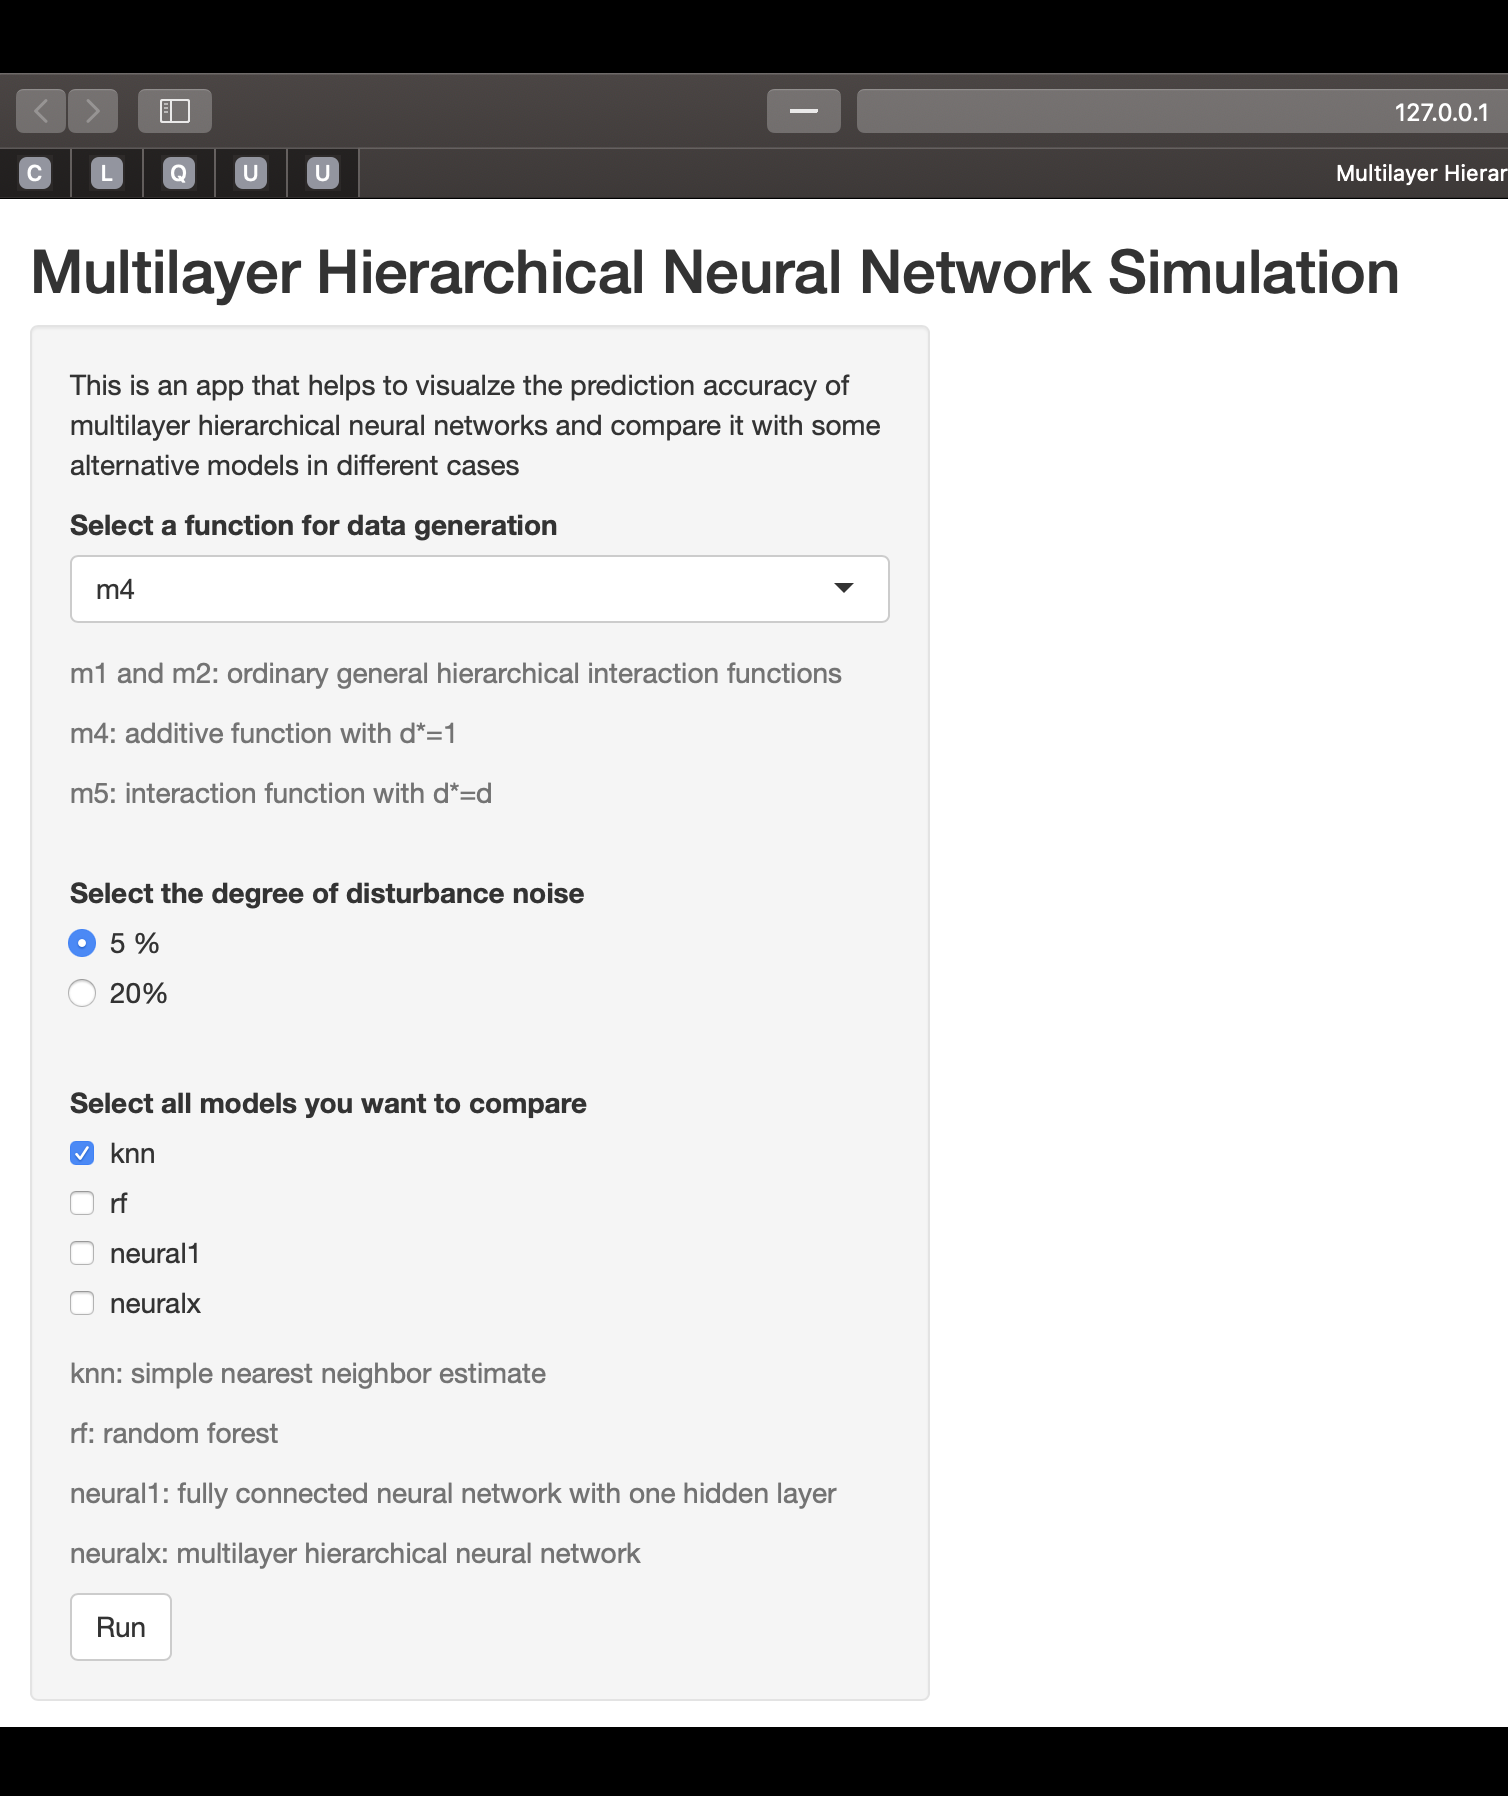
\includegraphics[scale=0.65]{figure3.png}
  \caption{Snapshot of R Shiny App}
  \label{fig3}
\end{figure}

\clearpage
\newpage

\begin{figure}[hp]
  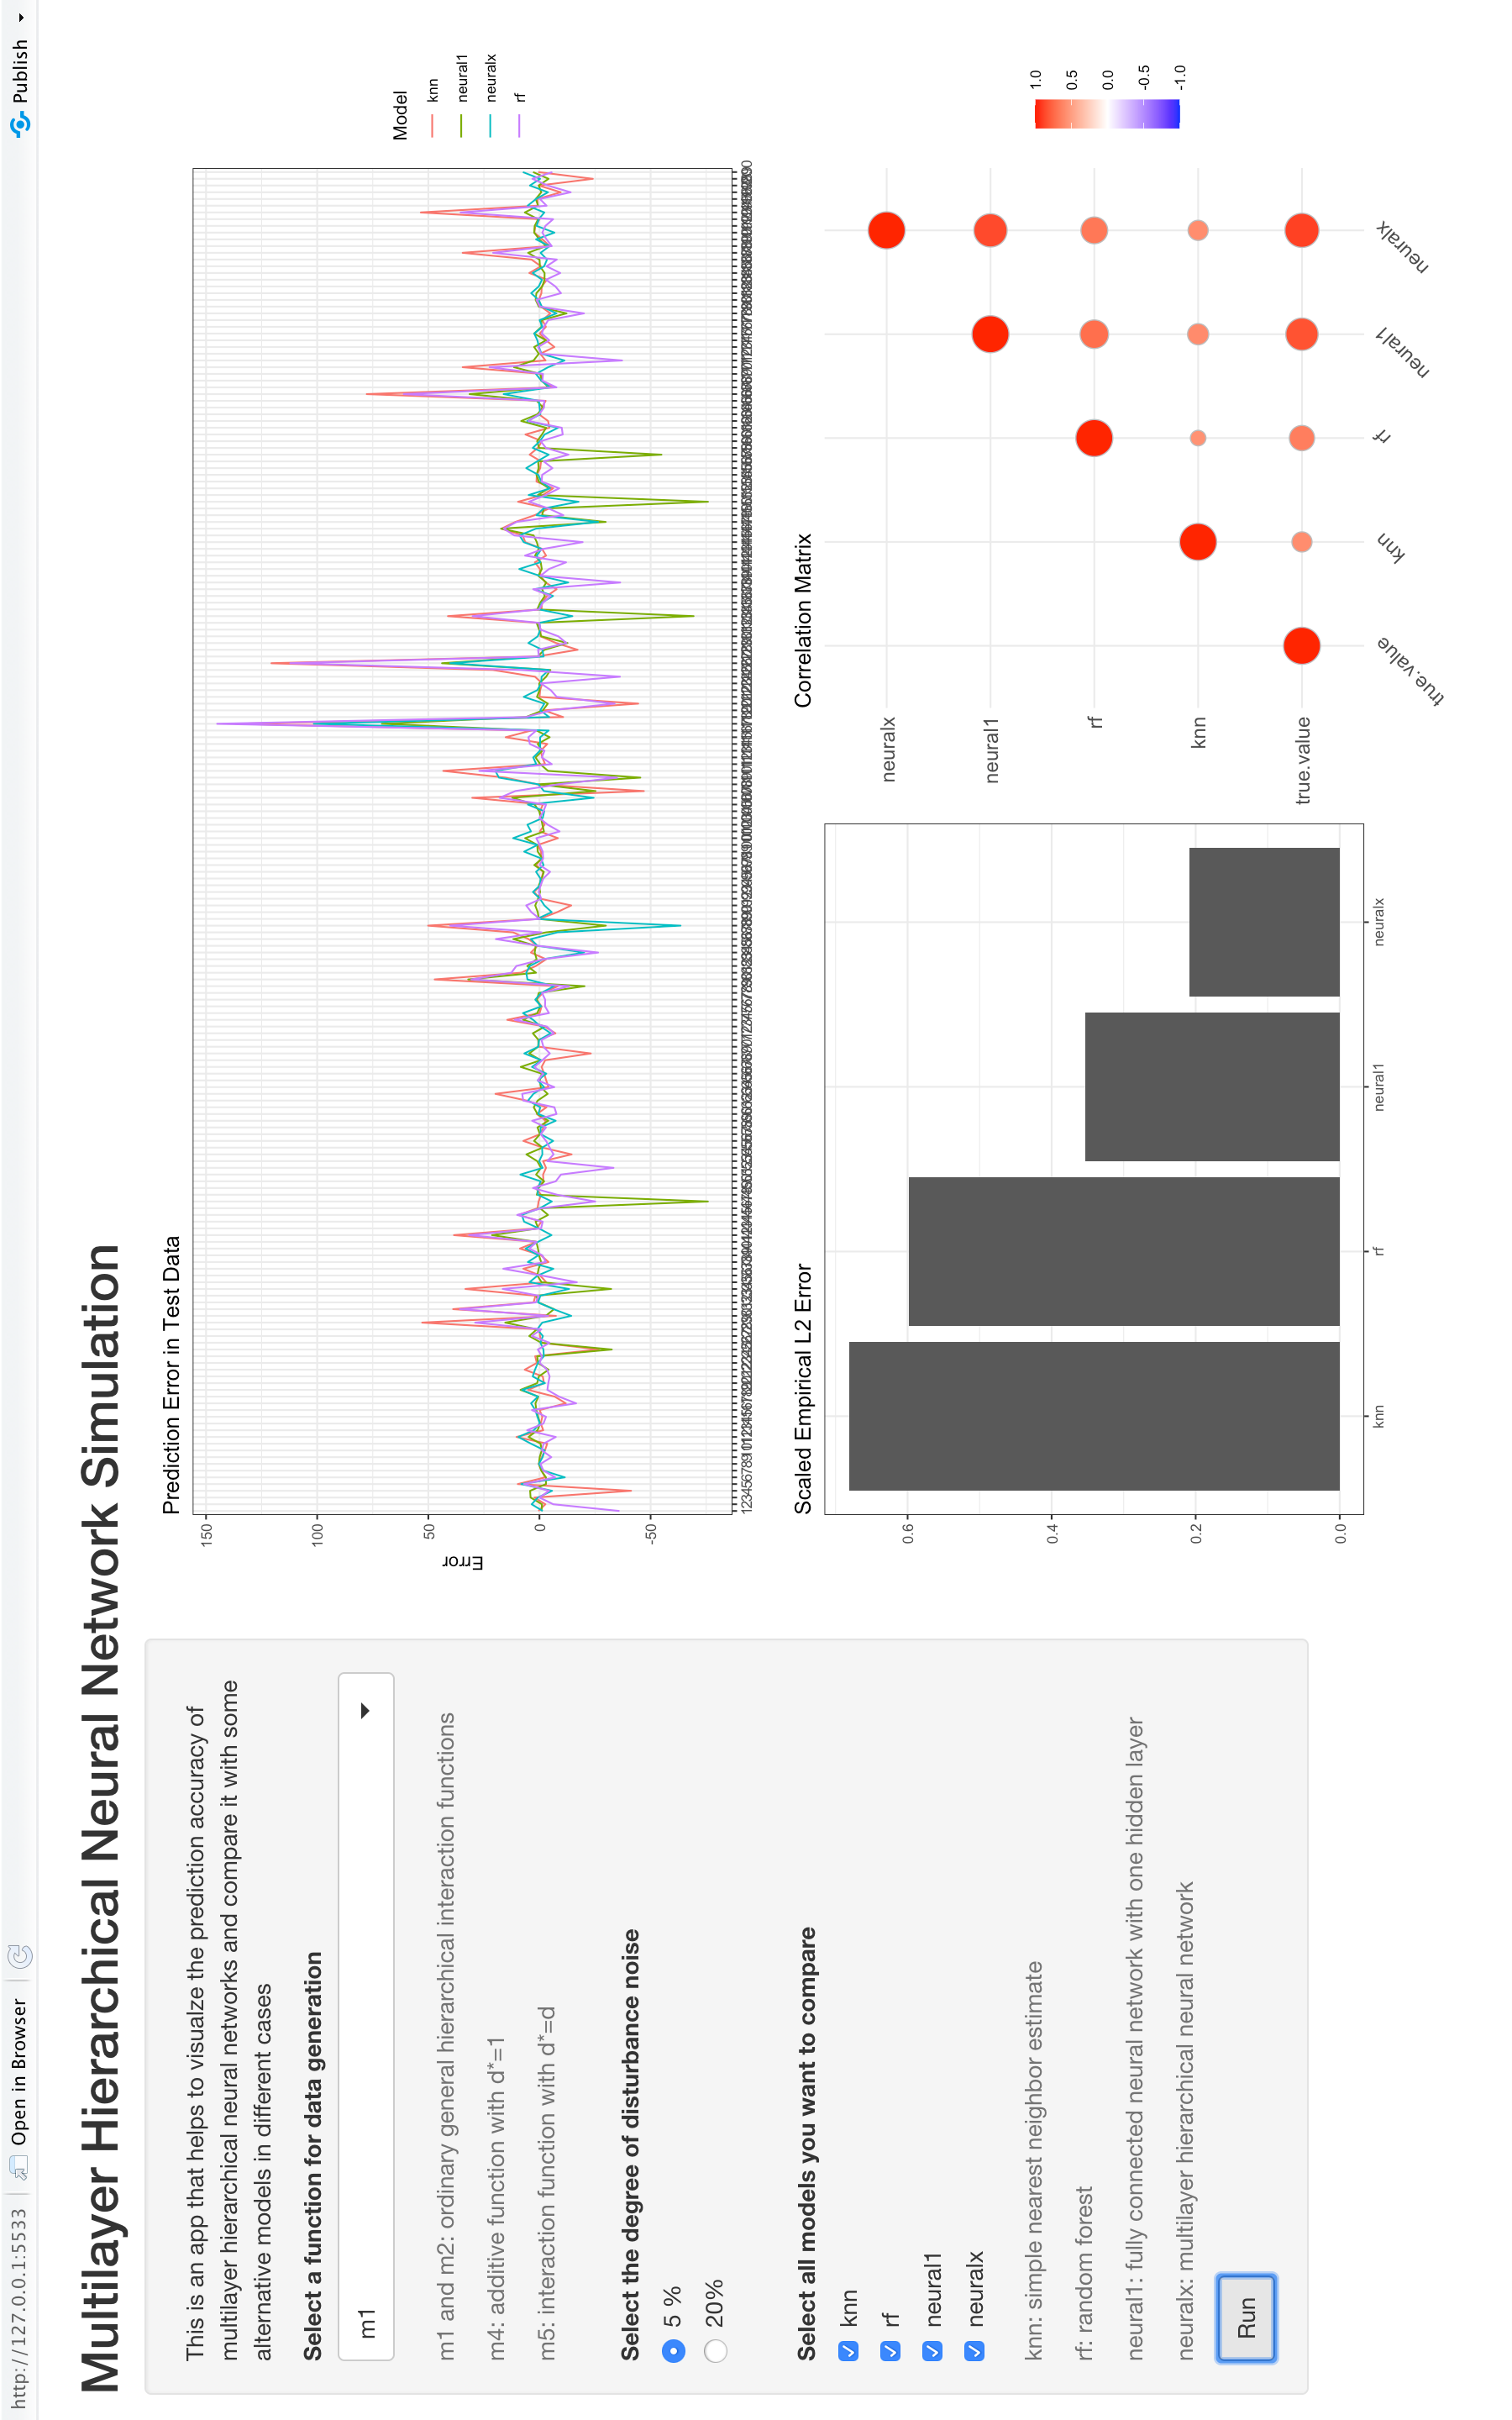
\includegraphics[scale=0.45]{figure4.png}
  \caption{Example of Outputs}
  \label{fig4}
\end{figure}

\clearpage



\printbibliography
\end{document}